\chapter{Background}
\label{back}
\section{ Who are the main participants in this product?}
ETH is used by individuals, Developor and enterprises.
\section{ Where are they from?}
The advantage of using ETH over more traditional currency is that it allows direct transfer of funds without any intermediate parties thus, reducing transaction fees. In addition, ETH also allows for more accessible banking services for example borrowing. 

ETH is extremely secure and private, applications created on the ethereum network protect user information from third parties. Governments or companies are unable to censor information on the ETH network as it is decentralised.

Developers use ETH to create applications and smart contracts. A smart contract is a computer program executed under some pre-specified conditions by the parties. For example, an individual may wish to purchase items online. Said individual can send funds to a smart contract then once the items have arrived at the individual doorstep the postman may scan the item and the funds will be released to the sender.

Enterprises see if ETH favourably because it provides a secure network for business operations such as making payments. ETH provides a protocol infersturce for tasks such as issuing or verifying credentials and allows for features enabling privacy, permissioning and performance.  \cite{eth}

Big banks, tech giants, and other organizations including J.P. Morgan Chase, Microsoft, and Intel are uniting to build business ready versions of the software behind Ethereum. Its ability to record and execute transactions without the need of a middleman is making this blockchain technology more popular amongst businesses. \cite{avatrade_2020}
 
\section{ What is their main agenda and what is their typical trading style?}
ETH can be used as a long-term investment and shorter term trading instruments.  Long-term investors will use ethereum to diversify their portfolios and engage in secure transactions without a middleman. In contrast to that short term traders seek to make profits in small movements of the price of ETH.  They will trade on Spot and derivative exchanges. Retail traders and institutions trade cryptos and their derivatives.

According to a recent report by coin news most parties that trade BTC are retail but professional traders dominate most of the market.  These professionals account for more than four fifths of all bitcoins sent to exchanges. \cite{retail}

\section{ What creates supply and demand for this asset?}
In addressing this question we will discuss the supply and demand of cryptos in general. 
Cryptocurrencies either have a limited or predetermined coin supply and so it is a deflationary asset. Since there is a limited supply of cryptocurrency this will increase demand and eventually drive prices up.

The main factors that drive supply in demand in the crypto market are media coverage, pumping and dumping schemes, marketing schemes, community support, trading bots, innovation and regulation. \cite{sd}
\begin{itemize}


\item Media coverage - 
Media coverage can bring awareness or influence the perception of certain cryptocurrencies in the market. For example a positive review of a cryptocurrency will have more buyers therefore, increasing price.

\item Pumping and Dumping - 
Pumping refers to a rise in price while dumping refers to a fall in price. 
Since prices are affected by supply and demand one can manipulate the prices via pumping and dumping schemes. A concentrated effort to match all the open orders on a particular crypto across several exchanges will create an artificial shortage. When the market adjusts, the price shoots up. Large holders of that crypto can then cash in on the gains by dumping their coins, bringing the price down.

\item Marketing schemes -
Influencers can disseminate information about coins via various media outlets. If coins have a high coverage the market is more aware of their existence.  Hence, there will be more buyers driving the price up.  Price can also fall if the influencer disseminates negative information about the coin.

\item Community support - 
A cryptocurrency with good community support and a strong vision for the future will thrive in the crypto markets as the project will bring value to members of that community. 

\item Trading Bots - Trading bots are very easily scalable so a program can command many bots to artificially inflate or deflate the price of a certain cryptocurrency. 

\item Innovation - Developers can add new functionality to particular coins.  The new functionality will make the coin more valuable thus driving the price up.

\item Regulation - Governments have control about the rules of cryptocurrency trading within their country  hence impacting the utility of a certain coin.  For example the chinese government has banned ICOs and Chinese based financial institutions are not allowed to deal in or fund cryptocurrencies. 
\end{itemize}

\section{What's are the tick increments and contract specifications for this product?}
For the ETH-PERPETUAL Deribit contract the tick increments are 5 cents.

The lists below show the product specifications for ETH traded products.
\subsection{Deribit ETH-PERPETUAL \cite{perp}}
\begin{itemize}
\item Underlying Asset/Ticker - Deribit ETH Index 
 
\item Contract - 1 USD per Index Point, with contract size USD 1 
 
\item Trading Hours - 24/7 
 
\item Minimum Tick Size - 0.05 USD

\item Settlement - Settlements take place every day at 8:00 UTC. Realized and unrealized session profits (profits made between settlements) are always added in real-time to the equity, however, they are only available for withdrawal after the daily settlement. At the settlement, session profits/losses will be booked to the ETH cash balance.

\item Contract Size - 1 USD
 
\item Initial Margin - The initial margin starts with $2.0 \%$ (50x leverage trading) and linearly increases by $1 \%$ per 5,000 ETH increase in the position size.
For example
 

Initial margin = $2.0 \%  + $(Position Size in ETH) $ * 0.0002\%$ 
 
\item Maintenance Margin - 	
The maintenance margin starts with $1 \%$ and linearly increases by $1 \%$ per 5,000 ETH increase in the position size.
 
\item Mark Price - The mark price is the price at which the perpetual contract will be valued during the trading hours. This can (temporarily) vary from the actual perpetual market price in order to protect market participants against manipulative trading.

Mark Price $=$ Index price + 30 seconds EMA of (Perpetual Fair Price $-$ Index Price)


The perpetual fair price is the average of bid and ask price for 1 ETH size order
 
\item Delivery/Expiration - No Delivery / Expiration
 
\item Fees maker - $0.00\%$, taker - $0.05\%$. However, for cryptoprop traders the maker rebate is $0.01 \%$ while the taker fee is $0.037\%$.
 
\item Position Limit - Maximum allowed position is 10,000,000 contracts (USD 10,000,000). Portfolio margin users are excluded from this limit and can build up larger positions. On request, the position limit could be raised based on an account evaluation.
 
\end{itemize} 
\subsection{Deribit Eth futures \cite{fut}}
\begin{itemize}


\item Underlying Asset/Ticker - Deribit ETH Index

\item 1 USD per Index Point, with contract size USD 1

\item Trading Hours - 24/7

\item Minimum Tick Size - 0.05 USD

\item Settlement - Settlements take place every day at 8:00 UTC. Realized and unrealized session profits (profits made between settlements) are always added in real-time to the equity, however, they are only available for withdrawal after the daily settlement. At the settlement, session profits/losses will be booked to the ETH cash balance.

\item Expiration Dates - Expirations always take place at 08:00 UTC, on the last Friday of the month. Currently, there are 3 quarterly futures (Expiring the last Friday of March, June, September, and December). A new future with a new expiry date will be added 1 hour before the expiry of the front future.

\item Contract Size - 1 USD

\item Initial Margin - 
The initial margin starts with 2.0% (50x leverage trading) and linearly increases by 1.0% per 5,000 ETH increase in position size.

Initial margin = $2\%$ + (Position Size in ETH) $* 0.0002\%$

\item Maintenance Margin - 
The maintenance margin starts with 1.0 $\%$ and linearly increases by 1.0$\%$ per 5,000 ETH increase in position size.

\item Mark Price - 
The mark price is the price at which the futures contract will be valued during trading hours. This can (temporarily) vary from the actual futures market price in order to protect market participants against manipulative trading.
Mark Price = Index price + 30 seconds EMA of (Futures Market Price - Index Price)
The market price is the last traded futures price if it falls between the current best bid and the best ask.  
Otherwise, if the last traded price is lower then the best bid, the market price will be the best bid. If the last traded price is higher than the best ask, the market price will be the best ask.

\item Delivery/Expiration -Friday, 08:00 UTC.

\item Delivery price - Time-weighted average of Deribit ETH index as measured between 07:30 and 08:00 UTC.

\item Delivery Method - Cash settlement in ETH.

\item Fees - Check this page for Deribit fees.

\item Position Limit - The maximum allowed position is 5,000,000 contracts (USD 5,000,000). Portfolio margin users are excluded from this limit and can build up larger positions. On request, the position limit could be increased based on an account evaluation.

\item Block Trade - Minimum USD 100,000.00


\end{itemize}




























\section{ What other products are closely correlated?}
ETH is highly correlated with other coins that also have large market caps. Figure \ref{fig:corr} compares ETH with a section of other high market cap coins. Over time these coins achieve a correlation upward of 0.8.

Figure \ref{fig:corr} also shows correlation between ETH, Gas and the SPY. Gas and the SPY have lower correations than high market cap coins.
\begin{figure}\label{fig:corr}
\center
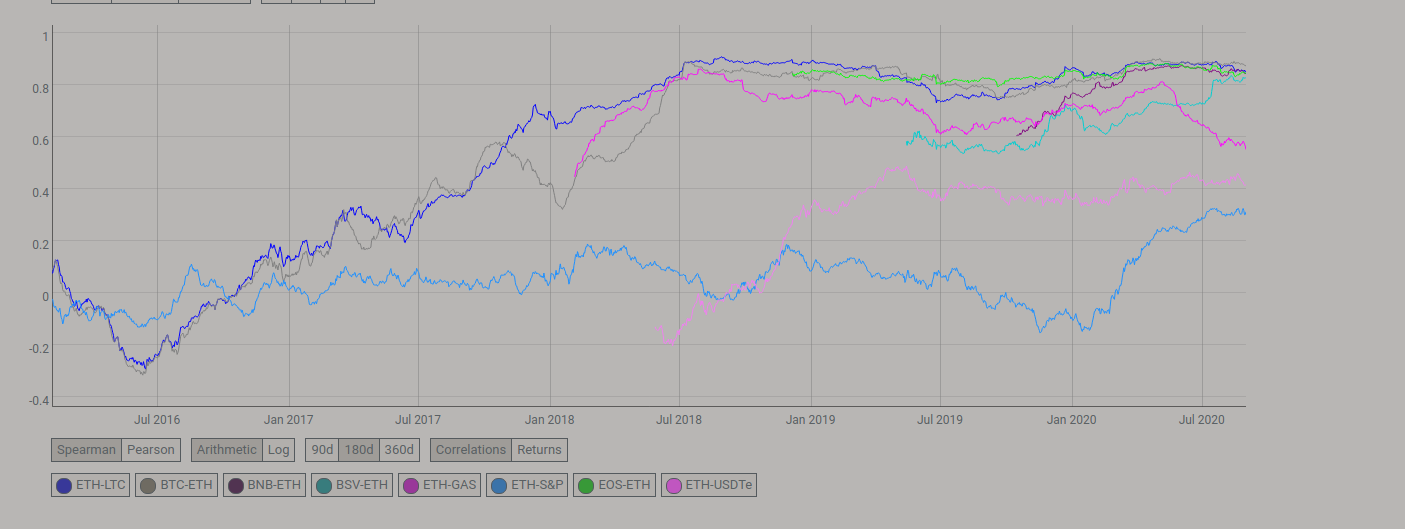
\includegraphics[width=0.95\textwidth]{fig/corrlations.png}
\caption{Screenshot from https://coinmetrics.io/. ETH correlation with LTC, BTC, BNB, BSV Gas, S\&P, EOS and USDTe for mid 2016 to mid 2020}
\end{figure}


\section{ Where is most of the volume done on this product? exchange, product type, future, perp etc}
Figure shows the percentage change, high low range and volume for the last 24 hours, 7 days and 30 days for futures exchanges.  The exchanges are ordered by volume. 
We see that with in each exchange a perpetual contract has more volume than a futures contract. HuobiDM has the most volume out of all the exchanges. Then in descending order of most volume is bybit, bitmex, deribit and finally binance.
\begin{figure}\label{fig:vol}
\center
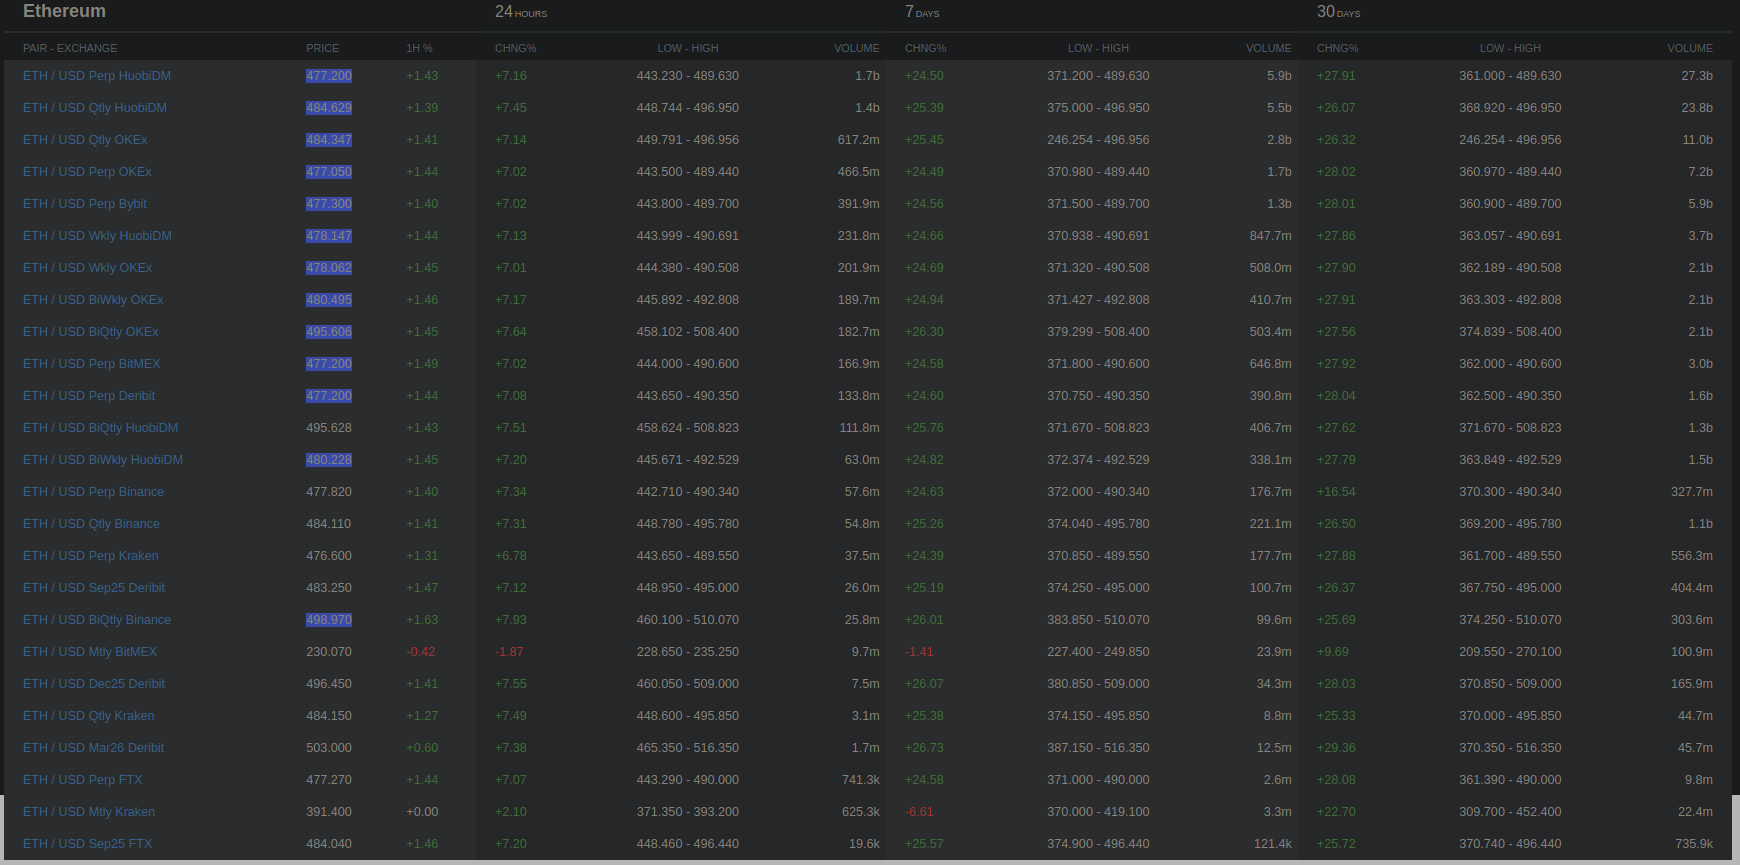
\includegraphics[width=0.95\textwidth]{fig/vol.png}
\caption{A screen shot taken from https://coinalyze.net/. Listed is the percentage change, high low range and volume for the last 24 hours, 7 days and 30 days for futures exchanges.  The exchanges are ordered by volume.}
\end{figure}
\section{ What is the mark price and how do you calculate it?}
Mark price is a reference price of a derivative that is calculated from underlying index. It will usually be a weighed moving average of the index spot price. The mark price is used so to avoid price manipulation of a single exchange. For the ETH-PERP on Deribit \cite{perp} the mark price is given by 


Mark Price = Index price + 30 seconds EMA of (Perpetual Market Price - Index Price)

\section{ Explain the effect of a positive funding rate on a long and short position.}
When the funding rate is positive, long position holders pay funding to the short position holders.

Below we show how the funding rate is calculated \cite{perp}

\begin{itemize}

\item Find the premium rate

Premium Rate = ((Mark Price - Deribit Index) / Deribit Index) * 100\%

\item The find the funding rate 

Funding Rate = Maximum (0.05\%, Premium Rate) + Minimum (-0.05\%, Premium Rate)

It should be noted that the funding rate is capped at $\pm 0.5\%$
\end{itemize}

If one wishes to find the funding payment, perform the addition steps

\begin{itemize}
\item calculate the time fraction

Time Fraction = Funding Rate Time Period / 8 hours

\item calculate the funding payment 

Funding Payment = Funding Rate * Position Size * Time Fraction
\end{itemize}
\section{ Explain the effect of a negative funding rate on a long and short position.}
When the funding rate is negative, short position holders pay funding to the long position holders.




\section{ If your account has 10BTC and you buy with 100,000 lots (\$) worth at the BTC price of 10,000 with 10x leverage. At what price will your account get liquidated? (keeping in mind your margin is in btc)}

Liquidations happen when there are no longer enough funds (margin) in your account to support your open positions. Your positions are then taken out of your control and closed (liquidated) by the platform. Another name for this is a margin call .Your positions will be liquidated when maintenance margin requirements get above your account equity \cite{liq}. 

It should be noted that account equity is calculated from the mark price of the instrument and not from the the last price.

Also extra fees are paid to close positions during the liquidations process. The fees go to the insurance fund.

For BTC the maintenance margin starts with 0.525\% and linearly increases by 0.5\% per 100 BTC increase in the position size. When the account's margin balance is lower than the maintenance margin, positions in the account will be incrementally reduced in order to keep the maintenance margin lower than the equity in the account. Maintenance margin requirements can be changed without prior notice if market circumstances demand such action.

 

Maintenance Margin= 0.525\% + (Position Size in BTC) * 0.005\%

\section{ Explain the difference between Deribit and Bitmex indices.}
    
    
    \section{ What is DeFi and what are the lead applications.}
    \section{ If you buy 100.000 bitmex contracts for Ethereum how much is that in \$?}
    \section{ What is a stop limit and what is a stop market order? Give an example of when and how each can be used.}